% Created 2014-11-06 Thu 03:26
\documentclass[11pt]{article}
\usepackage[utf8]{inputenc}
\usepackage[T1]{fontenc}
\usepackage{graphicx}
\usepackage{longtable}
\usepackage{float}
\usepackage{wrapfig}
\usepackage{soul}
\usepackage{amssymb}
\usepackage{hyperref}


\title{DataFlowAnalysis}
\author{miles}
\date{06 November 2014}

\begin{document}

\maketitle

\setcounter{tocdepth}{3}
\tableofcontents
\vspace*{1cm}
\section{Building \& Running}
\label{sec-1}

  Steps to build and run our DAMAJ Decaf Compiler.
  
  These instructions assume you are running on Athena.
  
  Clone the repository or otherwise obtain a copy of the code.

  Run \texttt{add -f scala}. use \texttt{scala -version} to make sure that scala is using version 2.11.2.
  We use \texttt{fsc} to compile scala a little faster. If you happen to have any trouble because of weird
  fsc version conflicts, please try killing your fsc server (find it with \texttt{ps aux | grep fsc}).
  Don't set any env variables like \texttt{SCALA\_HOME} as this could force you to use the wrong version
  of scala.
  
  Once you have the right version of scala run \texttt{make} or \texttt{build.sh} to compile the project.
  If you have trouble with this or later steps, try `make clean` to reset the build files.
  
  Now you should be able to run the compiler using run.sh.

  To enable optimizations you can add \texttt{-O all}.

  For example:

  \texttt{./run.sh --debug tests/codegen/input/01-callout.dcf -O all}

  \texttt{./run.sh --debug tests/codegen/input/04-math2.dcf -o 04-math2.asm}

  Alternatively, you can use \texttt{compile.sh} to compile and run a program.
  \texttt{./compile.sh tests/codegen/input/01-callout.dcf}
  This will assemble the program into \texttt{tmp/out.S}, print the assembly, create an executable at \texttt{tmp/out},
  and run the executable, printing its output as well.

\section{Dataflow Analyses}
\label{sec-2}

  Relevant files: \texttt{src/scala/dataflow/*}
  
  There is a trait \texttt{Analysis} from which all analyses inherit. It uses the worklist algorithm.
  Every analysis runs a transfer function on each block in a CFG. At this point in the analysis,
  every block contains at most one statement. Later, we will have analyses that run after condensing
  basic blocks in the CFG.

  Each type of analysis outputs an analysis result, parameterized by the specific type used for the analysis.

\subsection{Available Expressions}
\label{sec-2.1}

  Used in: Common Subexpression Elimination

  Operates on: Set of Expressions

  Available Expressions is a forward-running algorithm that determines whether each expression is available
  after each block. For every expression it sees, it checks whether the expression is pure. Right now, 
  every method call is declared not pure, but later we may have a finer-grained evaluation of method purity.

  If the expression is not pure, it is not a candidate for availability, its value is not cached, and all
  global variables are declared unavailable after the expression.

  If the expression is pure, then it becomes available.

  Whenever there is an assignment, the target of the assignment becomes unavailable, as do all expressions
  that use it.

\subsection{Live Variables}
\label{sec-2.2}

  Used in: Dead Code Elimination

  Operates on: Set of Variables.

  Live Variables Analysis is a backward-running algorithm that determines whether a variable will be used
  at each point in the program. 

  In every expression, every variable used in the expression is considered alive.

  The conditions of CFG forks are special-cased because otherwise the block that sets up the condition's
  temp variable will end up deleting it right before it is evaluated. This is because the condition of forks
  are not actually part of any block.

  In assignment statements, the destination of the assignment is no longer considered live (unless it is
  also in the right side of the assignment expression).

\subsection{Reachable}
\label{sec-2.3}

  Used in: Unreachable Code Elimination

  Operates on: Booleans

  Reachable is a forward-running algorithm that consideres a block unreachable if the output of the previous
  block was unreachable. A block's output becomes unreachable if it contains a return statement.

\subsection{Reaching Definitions}
\label{sec-2.4}

  Unused as of yet. Will be used for constant propagation.

  Operates on: Set of Assignment statements.

  Reaching definitions is a forward-running algorithm which determines which assignments are still used
  at a given point.

  For each assignment statement, previous assignments to the same variable are removed from the set,
  then the current assignment is added to the set.
  
\section{Optimizations}
\label{sec-3}

  When all optimizations are enabled, they run in the order presented below.

\subsection{Common Subexpression Elimination}
\label{sec-3.1}

    Operates on: Set of Expressions
    Available Expressions Analysis is a forward-running algorithm that determines wether an expressions variables are reassigned before the block. 
    Every assignment to x removes any expressions in the state that depend on variable x 
     
  Here is an example of CSE optimization. Please note that the blocks were given names for debugging 
  purposes, and that circular nodes are forking conditions.

  Before: 

  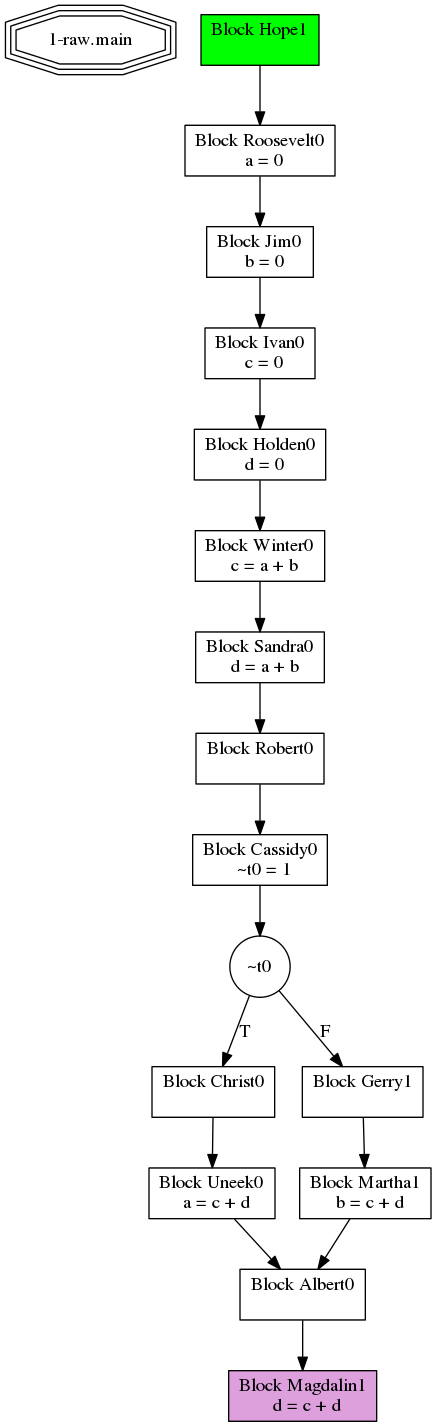
\includegraphics[width=0.4\textwidth]{./before_cse.png}
  
  After CSE:

  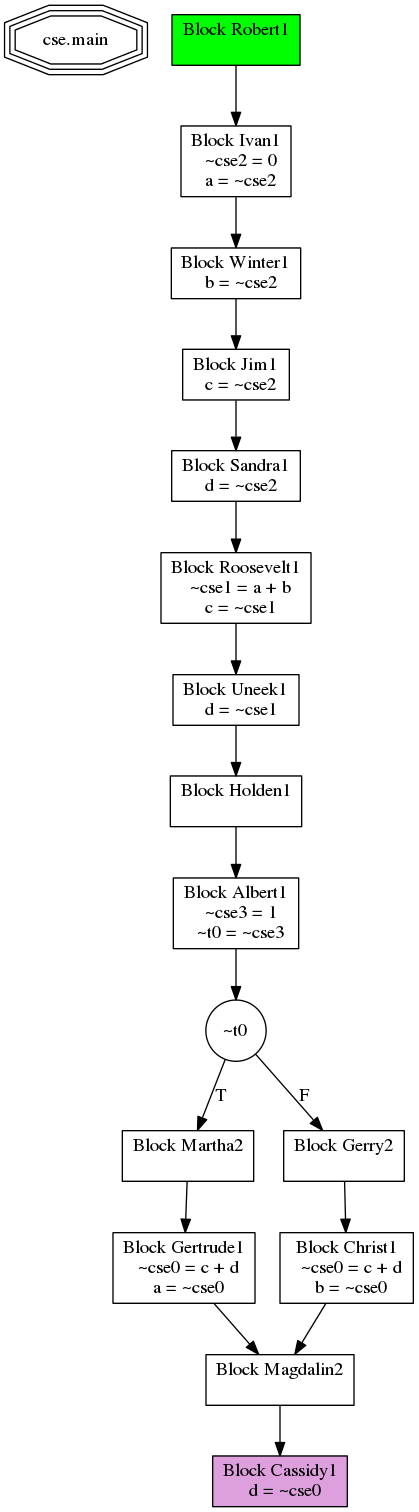
\includegraphics[width=0.4\textwidth]{./after_cse.png}

  Notice that CSE temps are generated for the expressions \texttt{0}, \texttt{a+b}, and \texttt{c+d}, and also that \texttt{c+d}
  appropriately is available for the last statement after it became available in each input branch. 

\subsection{Unreachable Code Elimination}
\label{sec-3.2}

    Unreachable code elimination, located in \texttt{src/scala/transform/UnreachableCodeElim.scala}, 
    deletes portions of code which can never be reached. It consumes the Reachable analysis. Any 
    block code deemed unreachable by Reachable is turned into a nop block with no statements. The 
    nop blocks are cleaned up in a later pass by the Condenser.

    Here is an example of UCE at work. Note that the blocks after the return in the if are not cleared because they could occur, but the blocks after the definitive return are cleared.

\subsection{Dead Code Elimination}
\label{sec-3.3}

  If there is an assignment to a dead variable, it is first checked for whether it is a method call. 
  If it is, it is converted simply to a method call without an assignment. Otherwise, the assignment
  to a dead variable is removed completely. 

  Here is an example of before and after Dead Code Elimination runs. Please note that the blocks were
  given names for debugging purposes, and that circular nodes are forking conditions.

  Before: 

  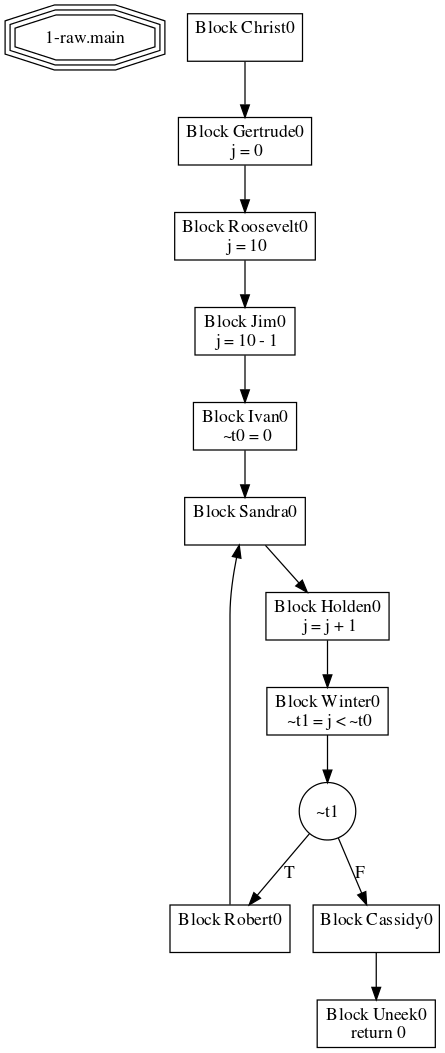
\includegraphics[width=0.4\textwidth]{./before_deadcode_example.png}
  
  After dead code elimination:

  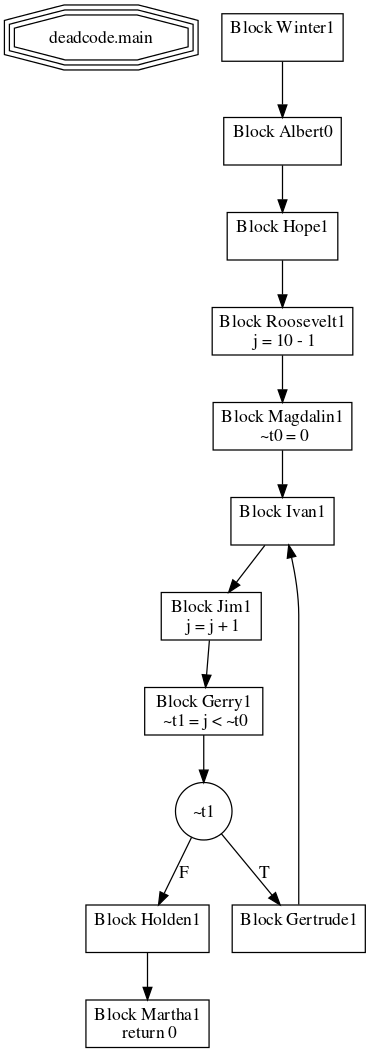
\includegraphics[width=0.4\textwidth]{./after_deadcode_example.png}

  Notice that the dead statements have been removed (the now-empty blocks will be removed in a later step).

\section{CFG Graph Generation}
\label{sec-4}

    A visual representation of the cfg we generate is a very useful debugging tool. 
    Graphiz is a simple and straightforward interface that takes a definition of graph, and
    produces a svg, pdf,png, or ps file with a visualization of the graph.
    We installed the dot package to show our directed graph
    To aid in debugging, we implemented a \texttt{grapher.scala} that takes in a CFG,
    and creates an output .gv (same as .dot) file.

\subsection{Generating Graphs}
\label{sec-4.1}

   First, make sure you have the `graphviz` package installed on your computer, which provides the program
   `dot`. Then, you can run `graph.sh` with the code. `graph.sh` takes all the same arguments that you can
   pass in to `run.sh`, so for example you could pass in only one optimization. It will generate a graph
   before and after each optimization pass, as well as generating annotated graphs for each analysis. 
   The last pass will condense blocks into more reasonable basic blocks.

   The graphs will be output in the `tmp` folder. 

   Try running:

   `./graph.sh -O all tests/dataflow/input/cse-01.dcf`

   And check out the output graphs!

\end{document}
